


For Wine and Housevotes datasets we found that a clustering with the Chebyshev distance produces clusterings with consideribly low scores for all evaluated indices. 
For Iris and Wine datasets ARI scores for the used \Gls{glos:K-Algorithms} have a peak for k=3 (\autoref{fig:comparison_iris}, \autoref{fig:comparison_wine}), which corresponds to the true number of labels in these datasets.  
By comparing different clustering algorithms for the Wine dataset \autoref{fig:comparison_wine} we found that the K-median algorithm is more unstable for this specific dataset than K-means and K-medoids as small peturbations of k can lead to remarkable differences in the resulting clustering scores. 

In our test cases the Angular Cosine distance always took the longest computation time for all clustering algorithms and datasets. The Euclidean distance had longer runtimes than Manhattan distance and Chebyshev distance. This is reasonable as for the Angular Cosine distance three sums and a square root need to be computed. The runtime for Euclidean distance is higher than for Manhattan or Chebyshev as a computation of an additional square root is necessary.\\
The fastest algorithm is DBSCAN, whereas K-Medoids takes the longest time to compute for all datasets besides Iris (where K-Medians with Cosine distance took extraordinary long). The runtime increases with the number of samples $n$ in the dataset. 

For the Iris dataset a clustering calculated by a K-algorithm (with k=3, \autoref{fig:comparison_iris}) with the Cosine distance gives the highest score values for all evaluated external scores. Therefore, the resulting clustering labels calculated with the Cosine distance evidentely match the true labels in the most accurate way in comparison with all other considered distance measures. Comparing the performances of all \Gls{glos:K-Algorithms} we found that K-medians and K-medoids give slightly higher scores than K-means. The results are very similar and differ only in a few differently assigned data points. \\
Using the Chebyshev distance for the Wine dataset results in clusterings with the lowest scores compared to all other distance measures. In contrast, k-means with the Euclidean distance and K-medians with the Manhattan distance perform relatively well for this dataset (\autoref{fig:comparison_wine}). However, the Chebyshev distance is not unsuitable for other datasets like the Iris dataset. Here, the distance performes similarly well as the other distance measures.
For the Diabetes dataset the K-medians algorithm with k=2 and the Manhattan distance performs the worst considering the Silhouette Score (\autoref{fig:comparison_diabetes}). The K-means algorithm along with the Euclidean, Manhattan or Cosine distance, as well as the results of the K-medians or K-medoids algorithm with Cosine distance, give the highest scoring results. A visual inspection of the t-SNE projected data points leads to an assumption of two main clusters in the data. Those clusters are well captured by a DBSCAN-Clustering with $eps = 0.1$ and $minPts = 4$, but not with a K-Algorithms-Clustering (\autoref{fig:diabetestsne}). Therefore we would suggest to use a DBSCAN-clustering approach for this dataset. 

\begin{figure}[H]
	\subfloat[DBSCAN ($eps = 0.1$ and $minPts = 4$)]{{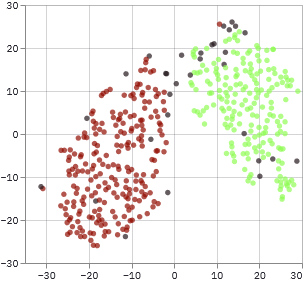
\includegraphics[width=0.45\textwidth]{./images/clustering_diabetes_dbscan_eps01_minpts4_tsne25} }}
	\subfloat[K-Means ($k=2$, Euclidean distance)]{{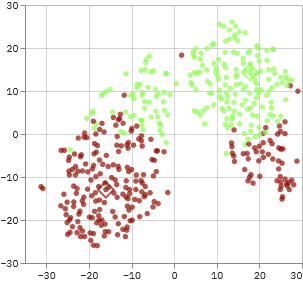
\includegraphics[width=0.45\textwidth]{./images/clustering_diabetes_kmeans_euclidean_k2_tsne25} }}  
	\caption{t-SNE projections of clustering results with DBSCAN and K-Means for Diabetes dataset}
	\label{fig:diabetestsne}
\end{figure}
 

For the Housevotes dataset (\autoref{fig:comparison_housevotes}) the Chebyshev distance performs the worst. The highest external scores for k=2 can be achieved with K-Means or K-Medians using the Euclidean,  Manhattan or Cosine distance. \\


In general, our study is restricted to a small set of algorithms and distance measures. As a result, it can only provide a limited overview. A variety of additional algorithms, distance metrics, parameter settings and cluster evaluation measures could be considered to get a more exhaustive in-depth analysis. By including more datasets a more detailed comparison of the algorithms and distance measures and their behaviour on differently distributed data might be possible. Furthermore, even more clustering indices, particularly internal indices, could give further insights on the clustering quality. \\

Finally, we did not find the best clustering algorithm or the superior distance measure which would give the best results on every dataset. This general problem in the field of Data Science is widely known as the "No Free Lunch Theorem" \cite{nofreelunch}. As specific requierements may differ for diverse use cases multiple algorithms and parameters should be explored and compared according to individual needs. 
